\documentclass[11pt]{scrartcl}
\usepackage[top=1cm, bottom=2.5cm, left=2.5cm, right=2.5cm]{geometry}
\usepackage{graphicx,float}
\usepackage{url}
\usepackage[T1]{fontenc}
\usepackage[font=small,labelfont=bf,tableposition=top]{caption}
\usepackage{amsmath,amssymb,amsfonts}
%\usepackage{algorithm, algorithmic}
%opening
\usepackage{titling}
\usepackage{multirow}
\setlength{\droptitle}{-2cm}
\title{Project Report 2}
\author{Fuyuan Lyu, Tianyu Shi, Dingyi Zhuang}

\begin{document}

\maketitle

\begin{abstract}
In this project, we try to implement different models based on \textit{scikit-learn} and other libraries and evaluate these models on two dataset: Twenty Newsgroup dataset, a multi-class classification task, and IMDB Reviews dataset, a binary classification task. When extracting feature vectors, we tried TF-IDF or used Glove embedding. We also tried to remove stop words or do Singular Value Decomposition (SVD) upon TF-IDF feature extractor. In the models implementation stage, we use models include but not limited to: SVM, Logistic Regression, Decision trees, Ada Boost, random forest, XGBoost, Multiple layer perceptron, LSTM. We also tune the hyper-parameter with greedy search method. SVM with TF-IDF techniques excels other upon Twenty Newsgroup dataset with 0.804 accuracy, IMDB dataset with 0.883 accuracy and overall 0.864 accuracy.
\end{abstract}

\section{Introduction}
The goal of this project is to investigate the performance of different models upon two different datasets: Twenty Newsgroup dataset and IMDB Reviews dataset and perform hyper-parameter tuning.

The Twenty Newsgroup dataset is a 20-class classification task with approximately 20000 newsgroup documents evenly spread\cite{Lang95}. While the IMDB Reviews dataset is a binary sentimental classification task with 25000 movie reviews for both training and testing\cite{maas-EtAl:2011:ACL-HLT2011}.

In the pre-processing stage, we mainly try two types of techniques. First is TF-IDF based counting features with different pre-processing tricks, such as removing stop word or SVD decomposition. Second is using pre-trained global vector representation to embed the word vector. Here we use GloVe, an unsupervised learning algorithm to obtain vector representation\cite{pennington2014glove}.

As for the model part, we try several different methods, include but not limited to: SVM, Logistic Regression (LR), Decision trees (DT), Ada Boost (ADB), random forest (RDF), XGBoost (XG), Multiple-layer perceptron(MLP) and LSTM-based neural network.

In the hyper-parameter tuning process, we separate the model into two categorizes. SVM, Logistic Regression, Decision trees, Ada Boost and random forest are tuned to improve performance. XGBoost, Multiple-layer perceptron and LSTM-based neural network are not tuned due to the lack of computation power.

Based on the result we obtained, TF-IDF is a more suitable preprocessing technique, SVM generally outperforms other models although its best parameters are different upon two datasets.


\section{Related Work}
Text classification intends to assign predefined labels to text documents \cite{allahyari2017brief,thangaraj2018text}. Firstly, probabilistic classifiers have gained a lot of popularity and shown markable performance \cite{chakrabarti1997using,joachims1996probabilistic,koller1997hierarchically,larkey1996combining}. These probabilistic methods introduce prior assumptions about how the data (words in documents) are generated and to use a probabilistic model on these assumptions. Besides probabilistic models, the hierarchical structures of decision trees is appealing. In the context of text data, the conditions on the trees nodes are usually defined as the terms in the documents, e.g. the presence or absence of a particular term in the document \cite{breiman1984classification,duda2012pattern}. Decision trees are also combined with boosting techniques to improve the accuracy of classification \cite{freund1995desicion,schapire2000boostexter}. Owing to the robustness of data, SVM are also widely implemented to form linear classifiers for supervised learning classification algorithms \cite{joachims1998text,joachims2001statistical}.

Multiple classes in text classification makes it difficult to pick a particular set of attributes. There are many evolving techniques that adapt the algorithms for multi-class task, including K-nearest neighbor, decision trees and SVM \cite{tang2016multi,yi2011multi}. Recently neural network is widely applied in hierarchical multi-label classification issues. Neural network forms the base of the ensemble with the help of composite stumps \cite{nie2015neural,cerri2014hierarchical}.


\section{Dataset and setup}
We use two dataset to test our model performance. The Twenty Newsgroup dataset is a 20-class classification task with approximately 20000 newsgroup documents evenly spread\cite{Lang95}. While the IMDB Reviews dataset is a binary sentimental classification task with 25000 movie reviews for both training and testing\cite{maas-EtAl:2011:ACL-HLT2011}. In the feature-extraction stage, we propose two types of methods: TF-IDF based and word2vec based. In the TF-IDF based method, we first tokenize every samples and apply TF-IDF to each. Several other feature engineering techniques, such as removing stop word or SVD decomposition. In the word2vec based method, we use pre-trained GloVe\cite{pennington2014glove} word representation to represent each sample.

\section{Proposed approach}
For our prediction model, we choose logistic regression , decision tree, support vector classifier, Adaboost, random forest, XGBoost and neural networks as candidate models. Of all the well-known learning methods, decision trees come closest to meeting the requirements for serving as an off-the-shelf procedure for data mining. They are relatively fast to construct and they produce interpretable models (if the trees are small). For naive bayes model, it does not require as much training data. Also, it is not sensitive to irrelevant features. For SVM model, It scales relatively well to high dimensional data. SVM models have generalization in practice, the risk of over-fitting is less in SVM. For XGBoost algorithm, it is a well-known tree boosting algorithm applied into many real world application. We choose MLP model because it is a very good algorithm to be used to map an N-dimensional input signal to an M-dimensional output signal, this mapping can also be non-linear. However, this will increase the total training time.  As these two datasets are sequence data, so we also leveraged the advantage of LSTM models for prediction.

\section{Results}

The experiments are performed to find a suitable preprocessing and classification technique for the proposal text documentation classifiers. Effect of different preprocessing methods (TF-IDF, stop words removal and SVD with different latent dimensions) on the performance of the classifiers along with grid-search on tuning parameters on each classifiers are also discussed. We combine $sklearn.pipline$ and $sklearn.model_selection.GridSearchCV$ to conduct general parameters search on 7 different data preprocessing methods where we choose $k=5$ for cross-validation when tuning parameters. 

\subsubsection*{Analysis of the accuracy performance of different classifiers}
We plot test accuracy of different classifiers on two datasets according to 7 preprocessing techniques, including TF-IDF, TF-IDF \& removing stopping words and TF-IDF \& SVD with latent dimensions from 2 to 6. The result is shown in Figure \ref{accuracy_20} and Figure \ref{accuracy_imdb}.

\begin{figure}[H]
	\centering
	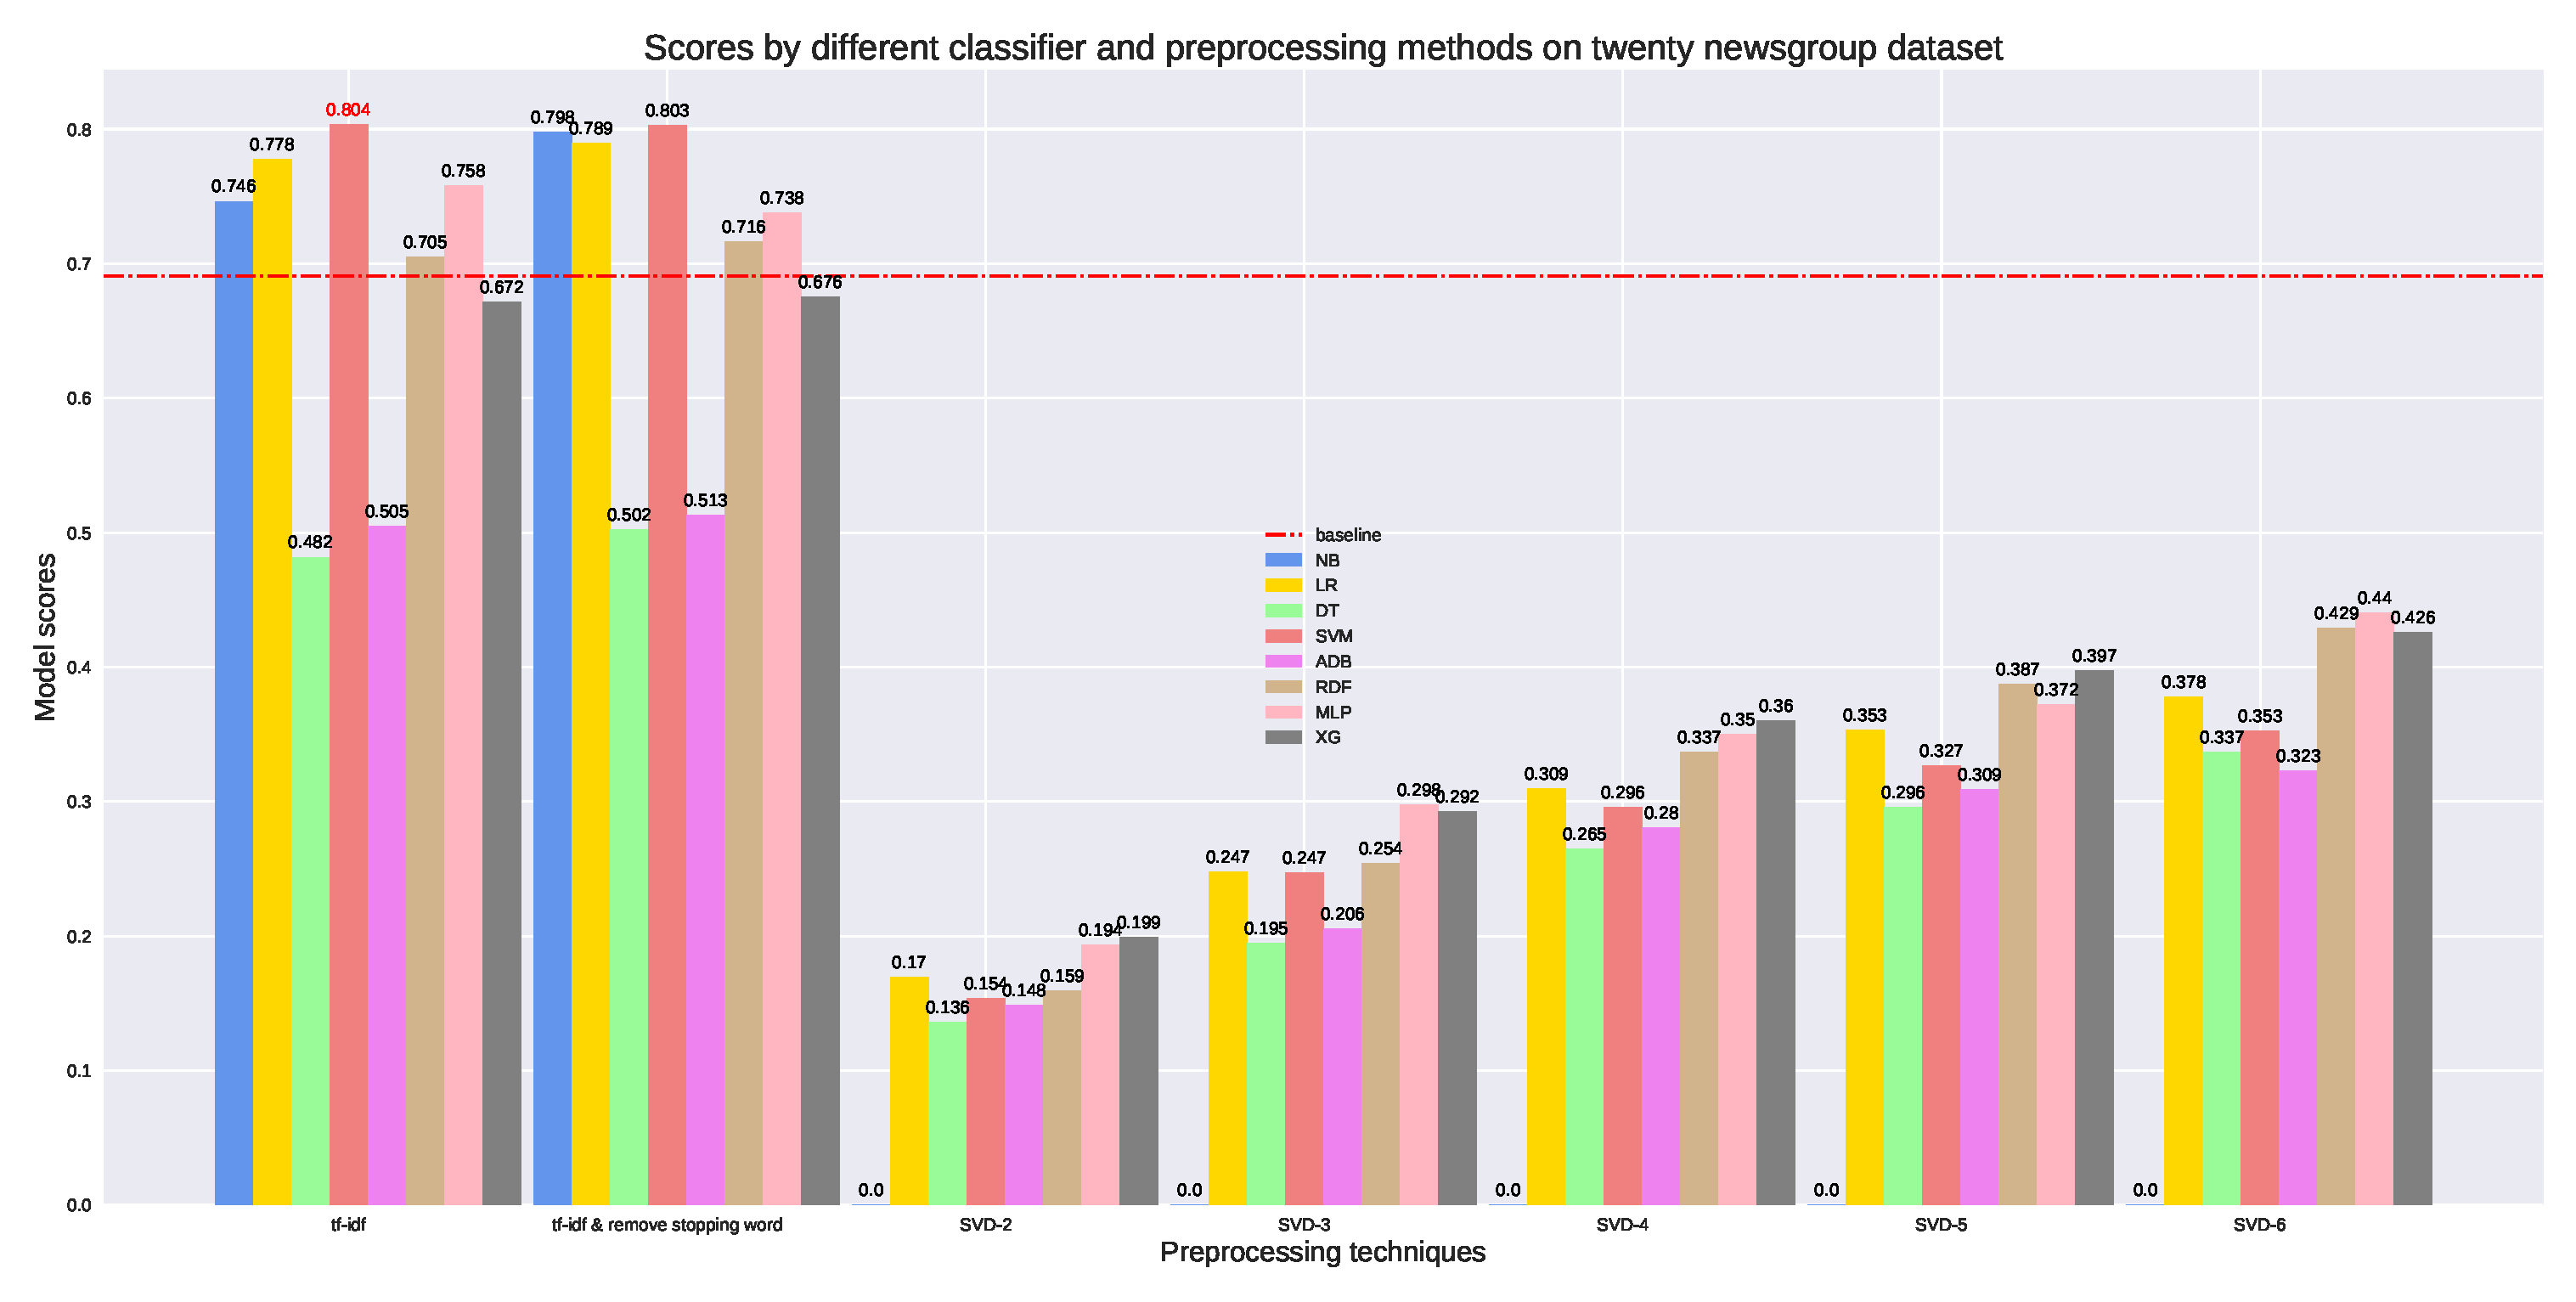
\includegraphics[width=0.9\linewidth]{fig/model_acc_20.eps}
	\caption{Classifiers accuracy on test dataset of Twenty Newsgroup dataset according to different pre-processing techniques}
	\label{accuracy_20}
\end{figure}

\begin{figure}[H]
	\centering
	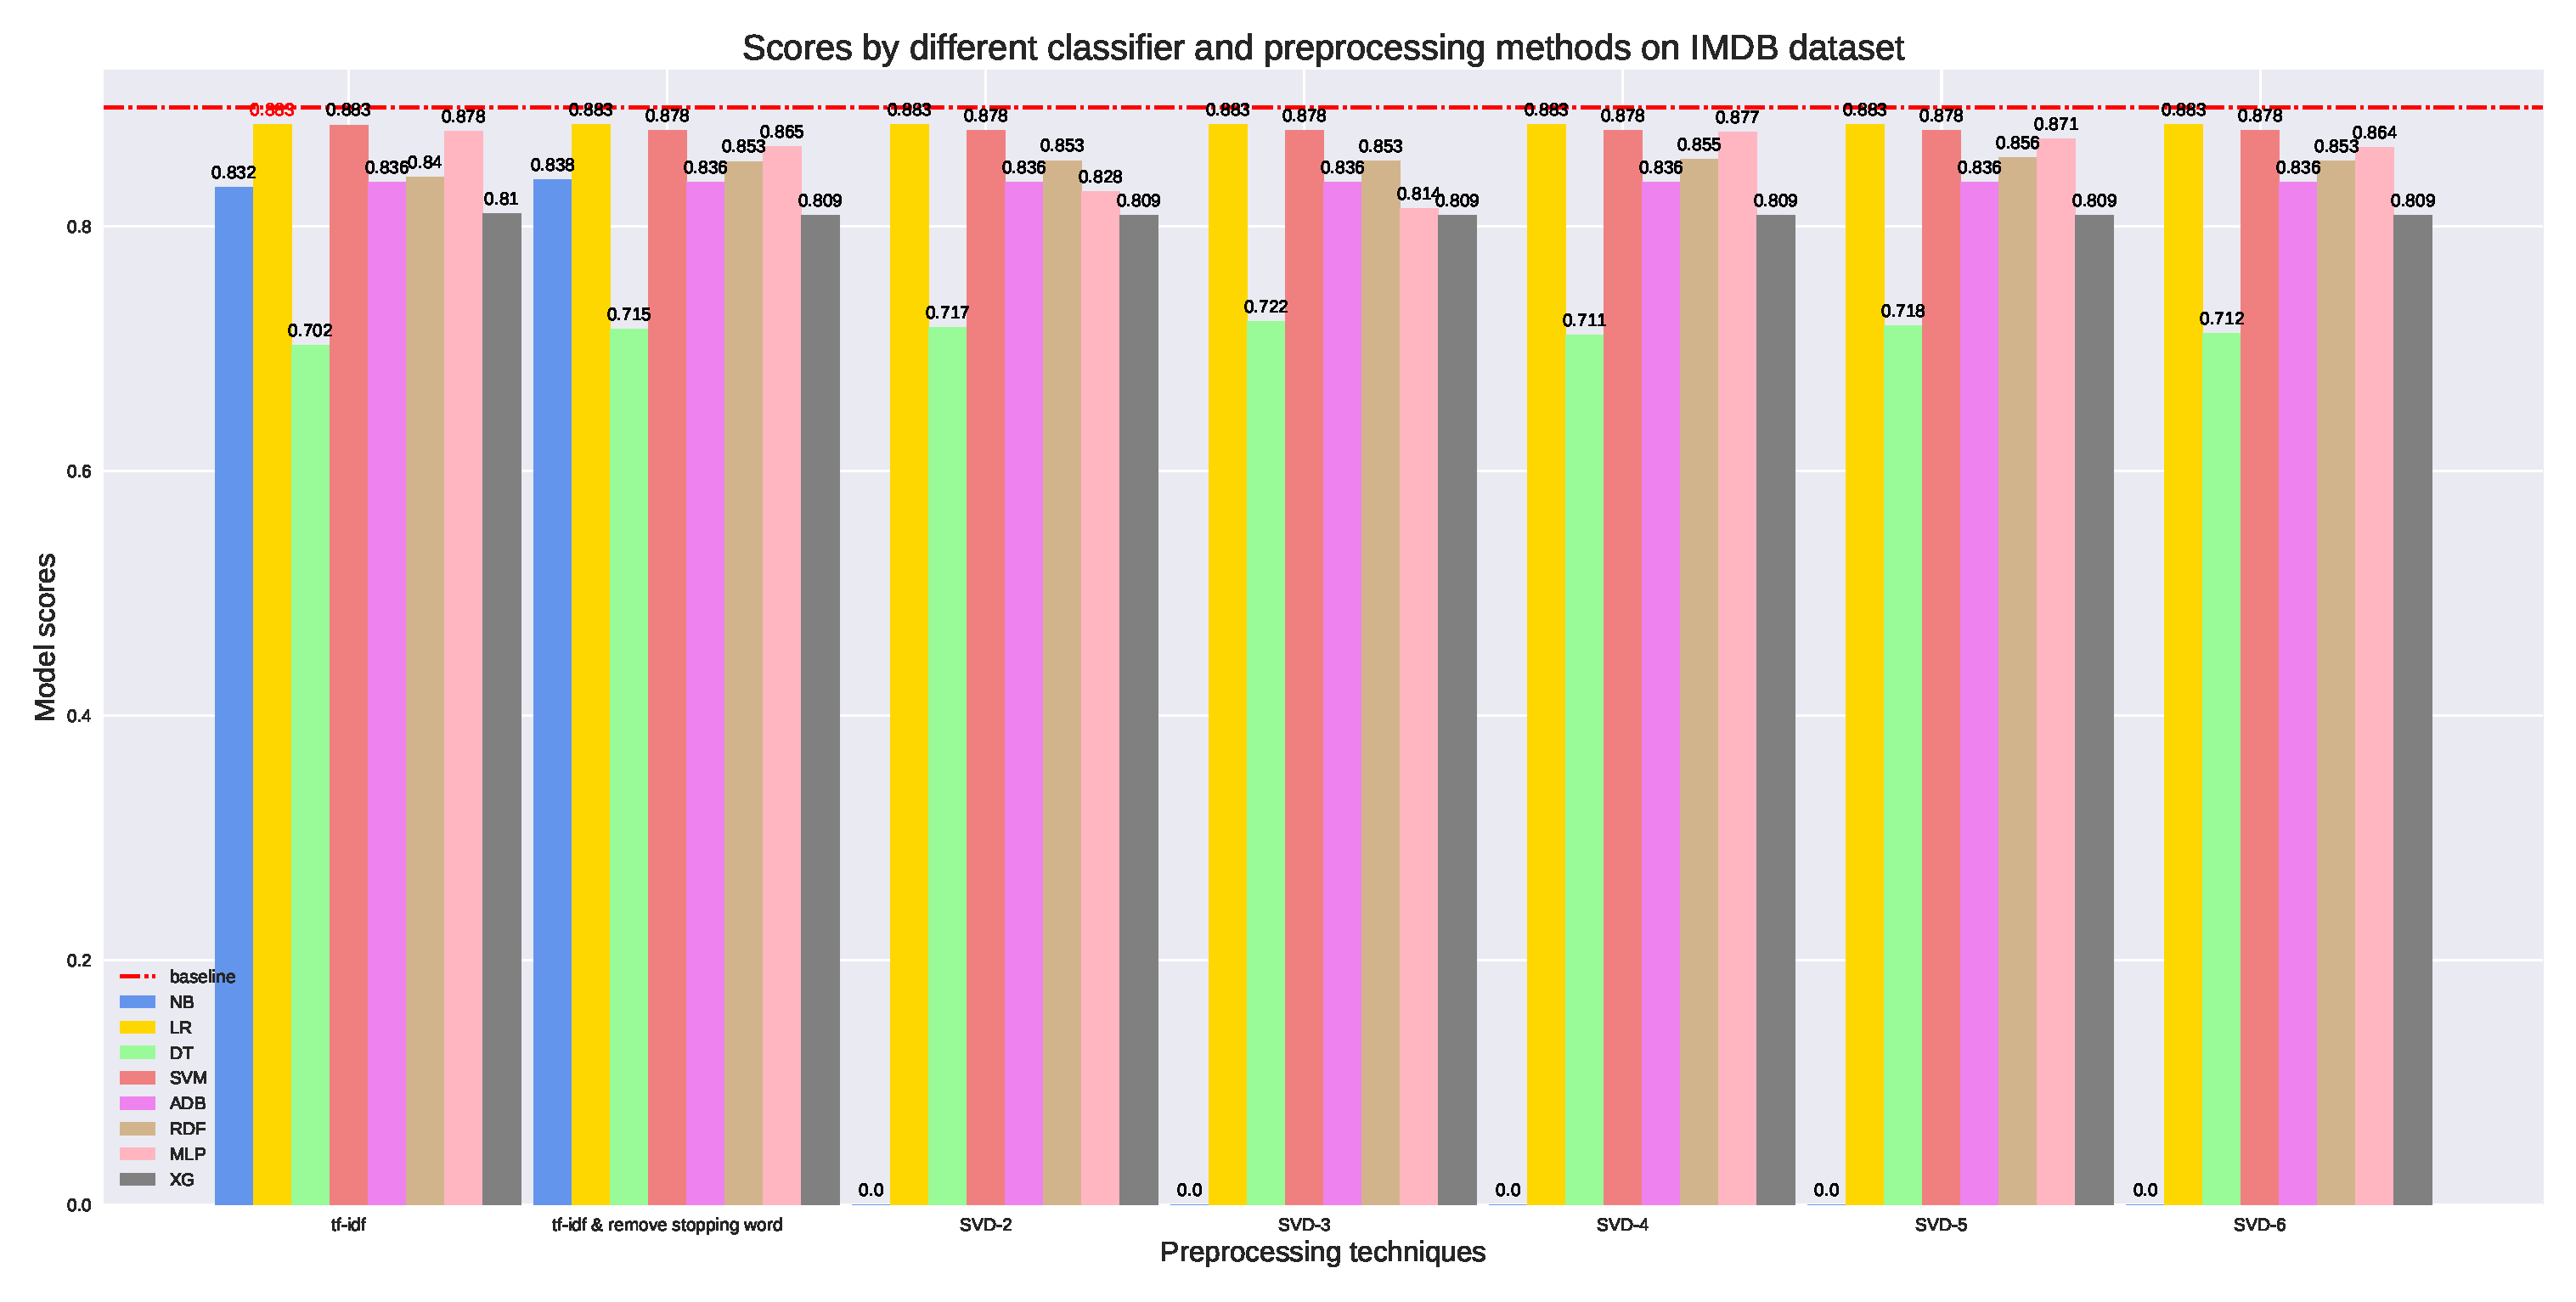
\includegraphics[width=0.9\linewidth]{fig/model_acc_imdb.eps}
	\caption{Classifiers accuracy on test dataset of IMDB according to different pre-processing techniques}
	\label{accuracy_imdb}
\end{figure}

The best performance is marked red. To be noticed that the SVD decomposition will produce negative values, which is not compatible for NB input. The accuracy and runtime plots would miss such records. From Figure \ref{accuracy_20}, it is clear dimensions reductions will lose much information if we focus on the multi-class classification problem like Twenty Newsgroup dataset but will slightly improve the performance of binary classifiers in Figure \ref{accuracy_imdb}. Generally, SVM performs best in both datasets, with accuracy 0.804 in TF-IDF processed Twenty Newsgroup dataset and 0.883 in TF-IDF processed IMDB dataset.

\subsubsection*{Analysis of the runtime performance of different classifiers}
Futhermore, We plot runtime of classifiers with best parameters on two datasets according to 7 preprocessing techniques, as shown in Figure \ref{runtime_20} and Figure \ref{runtime_imdb}.

\begin{figure}[H]
	\centering
	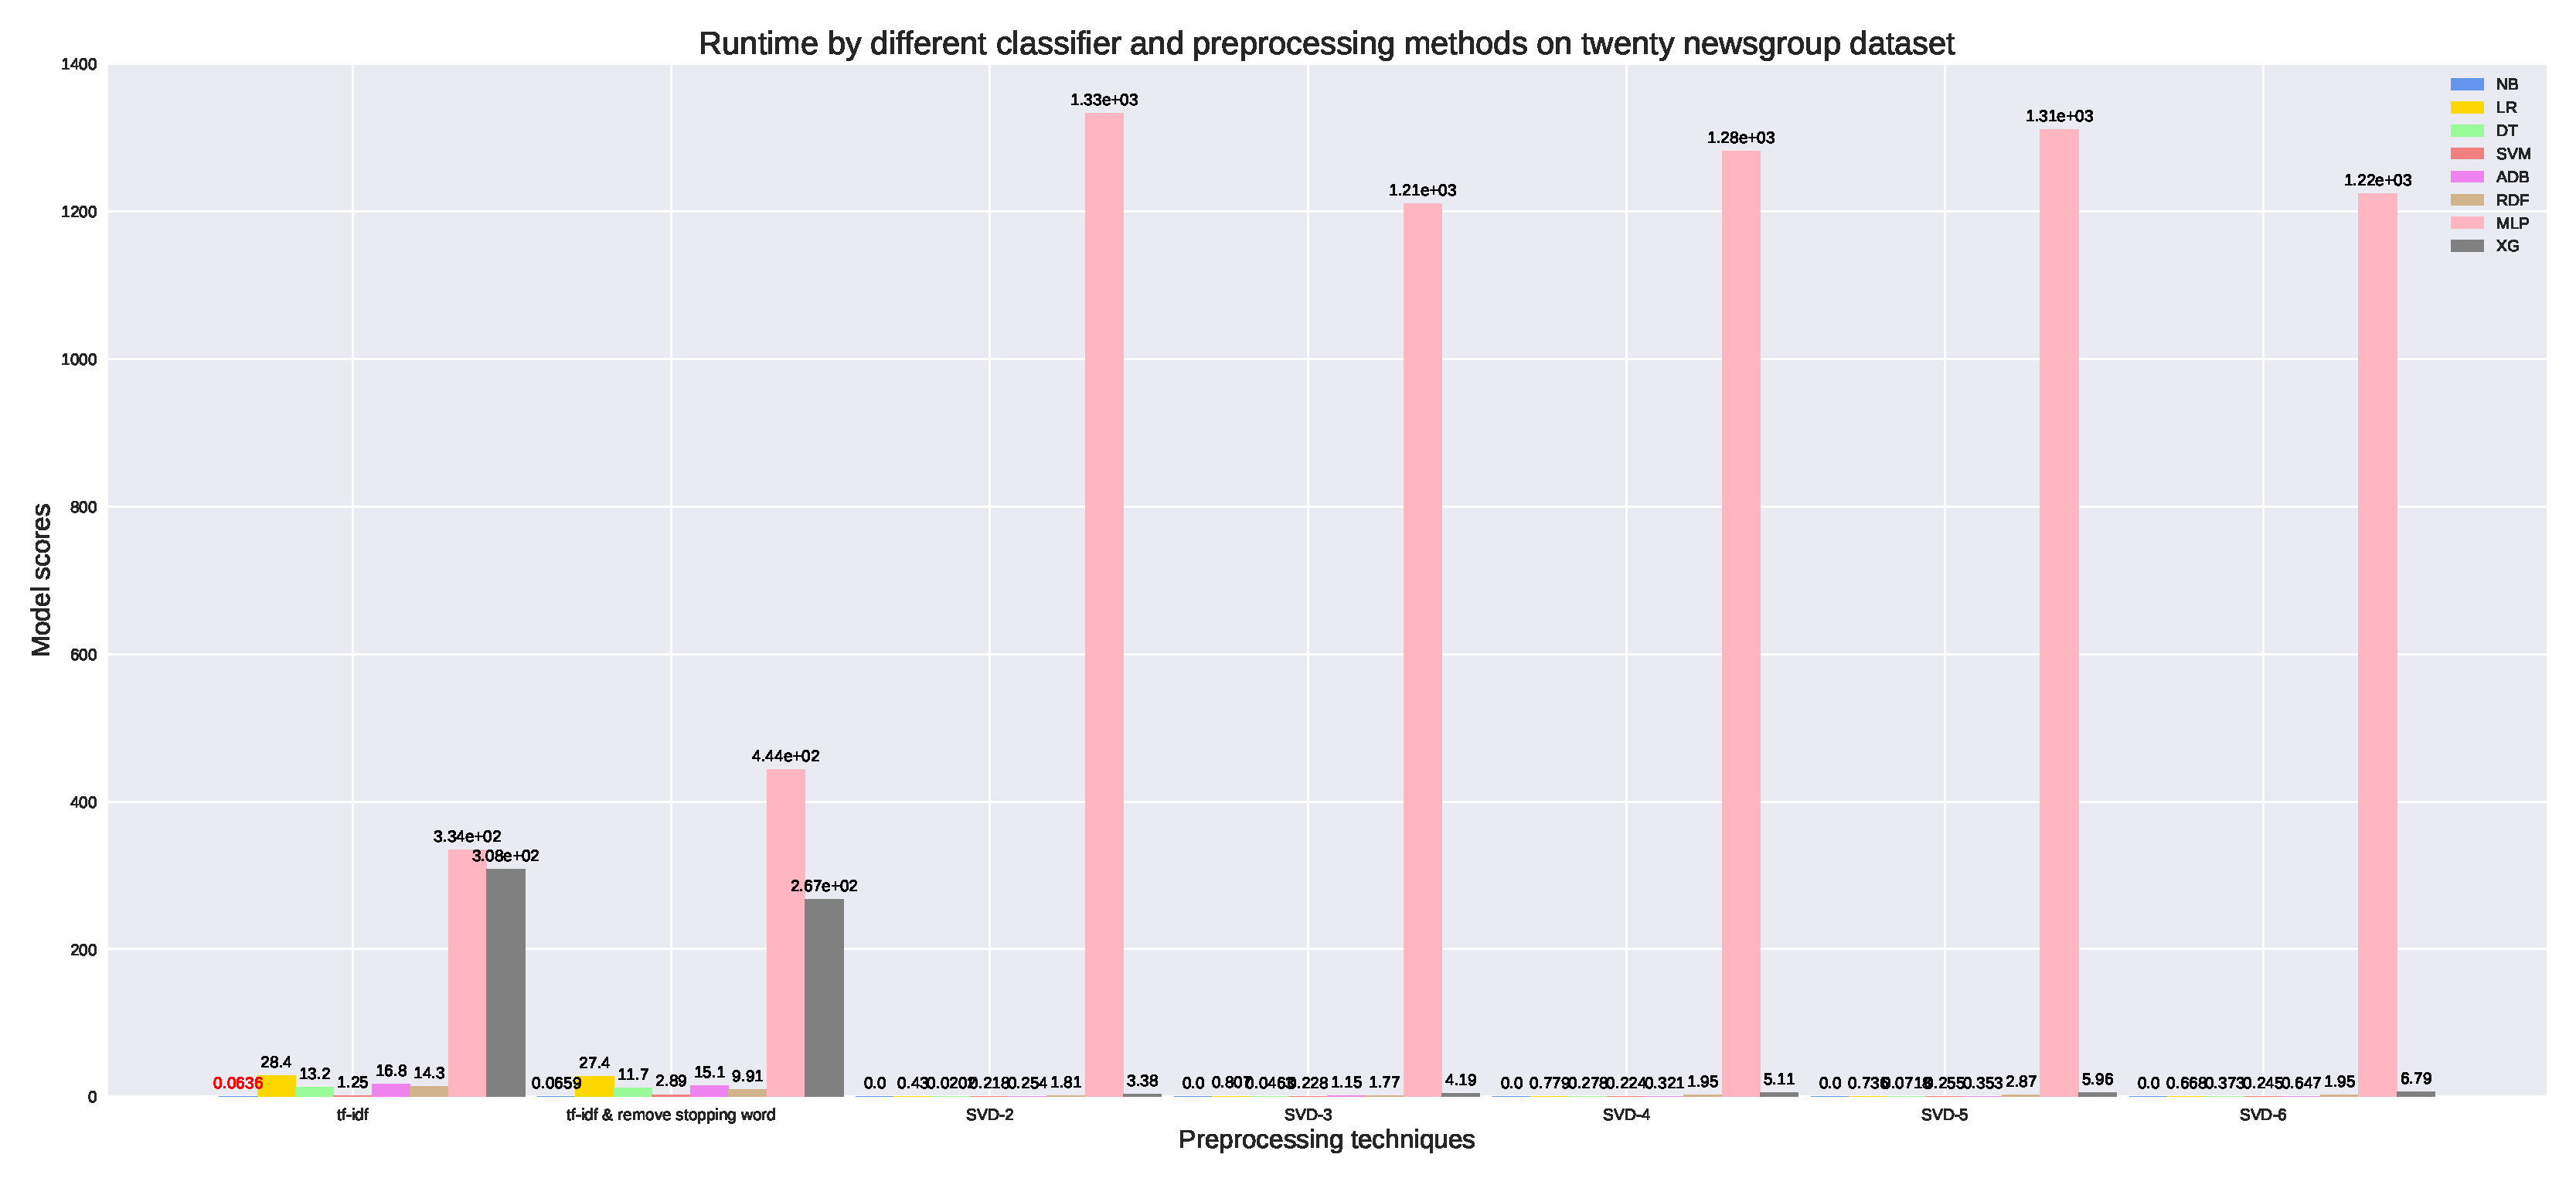
\includegraphics[width=0.9\linewidth]{fig/model_runtime_20.eps}
	\caption{Runtime performance on test dataset of Twenty Newsgroup dataset according to different pre-processing techniques}
	\label{runtime_20}
\end{figure}

\begin{figure}[H]
	\centering
	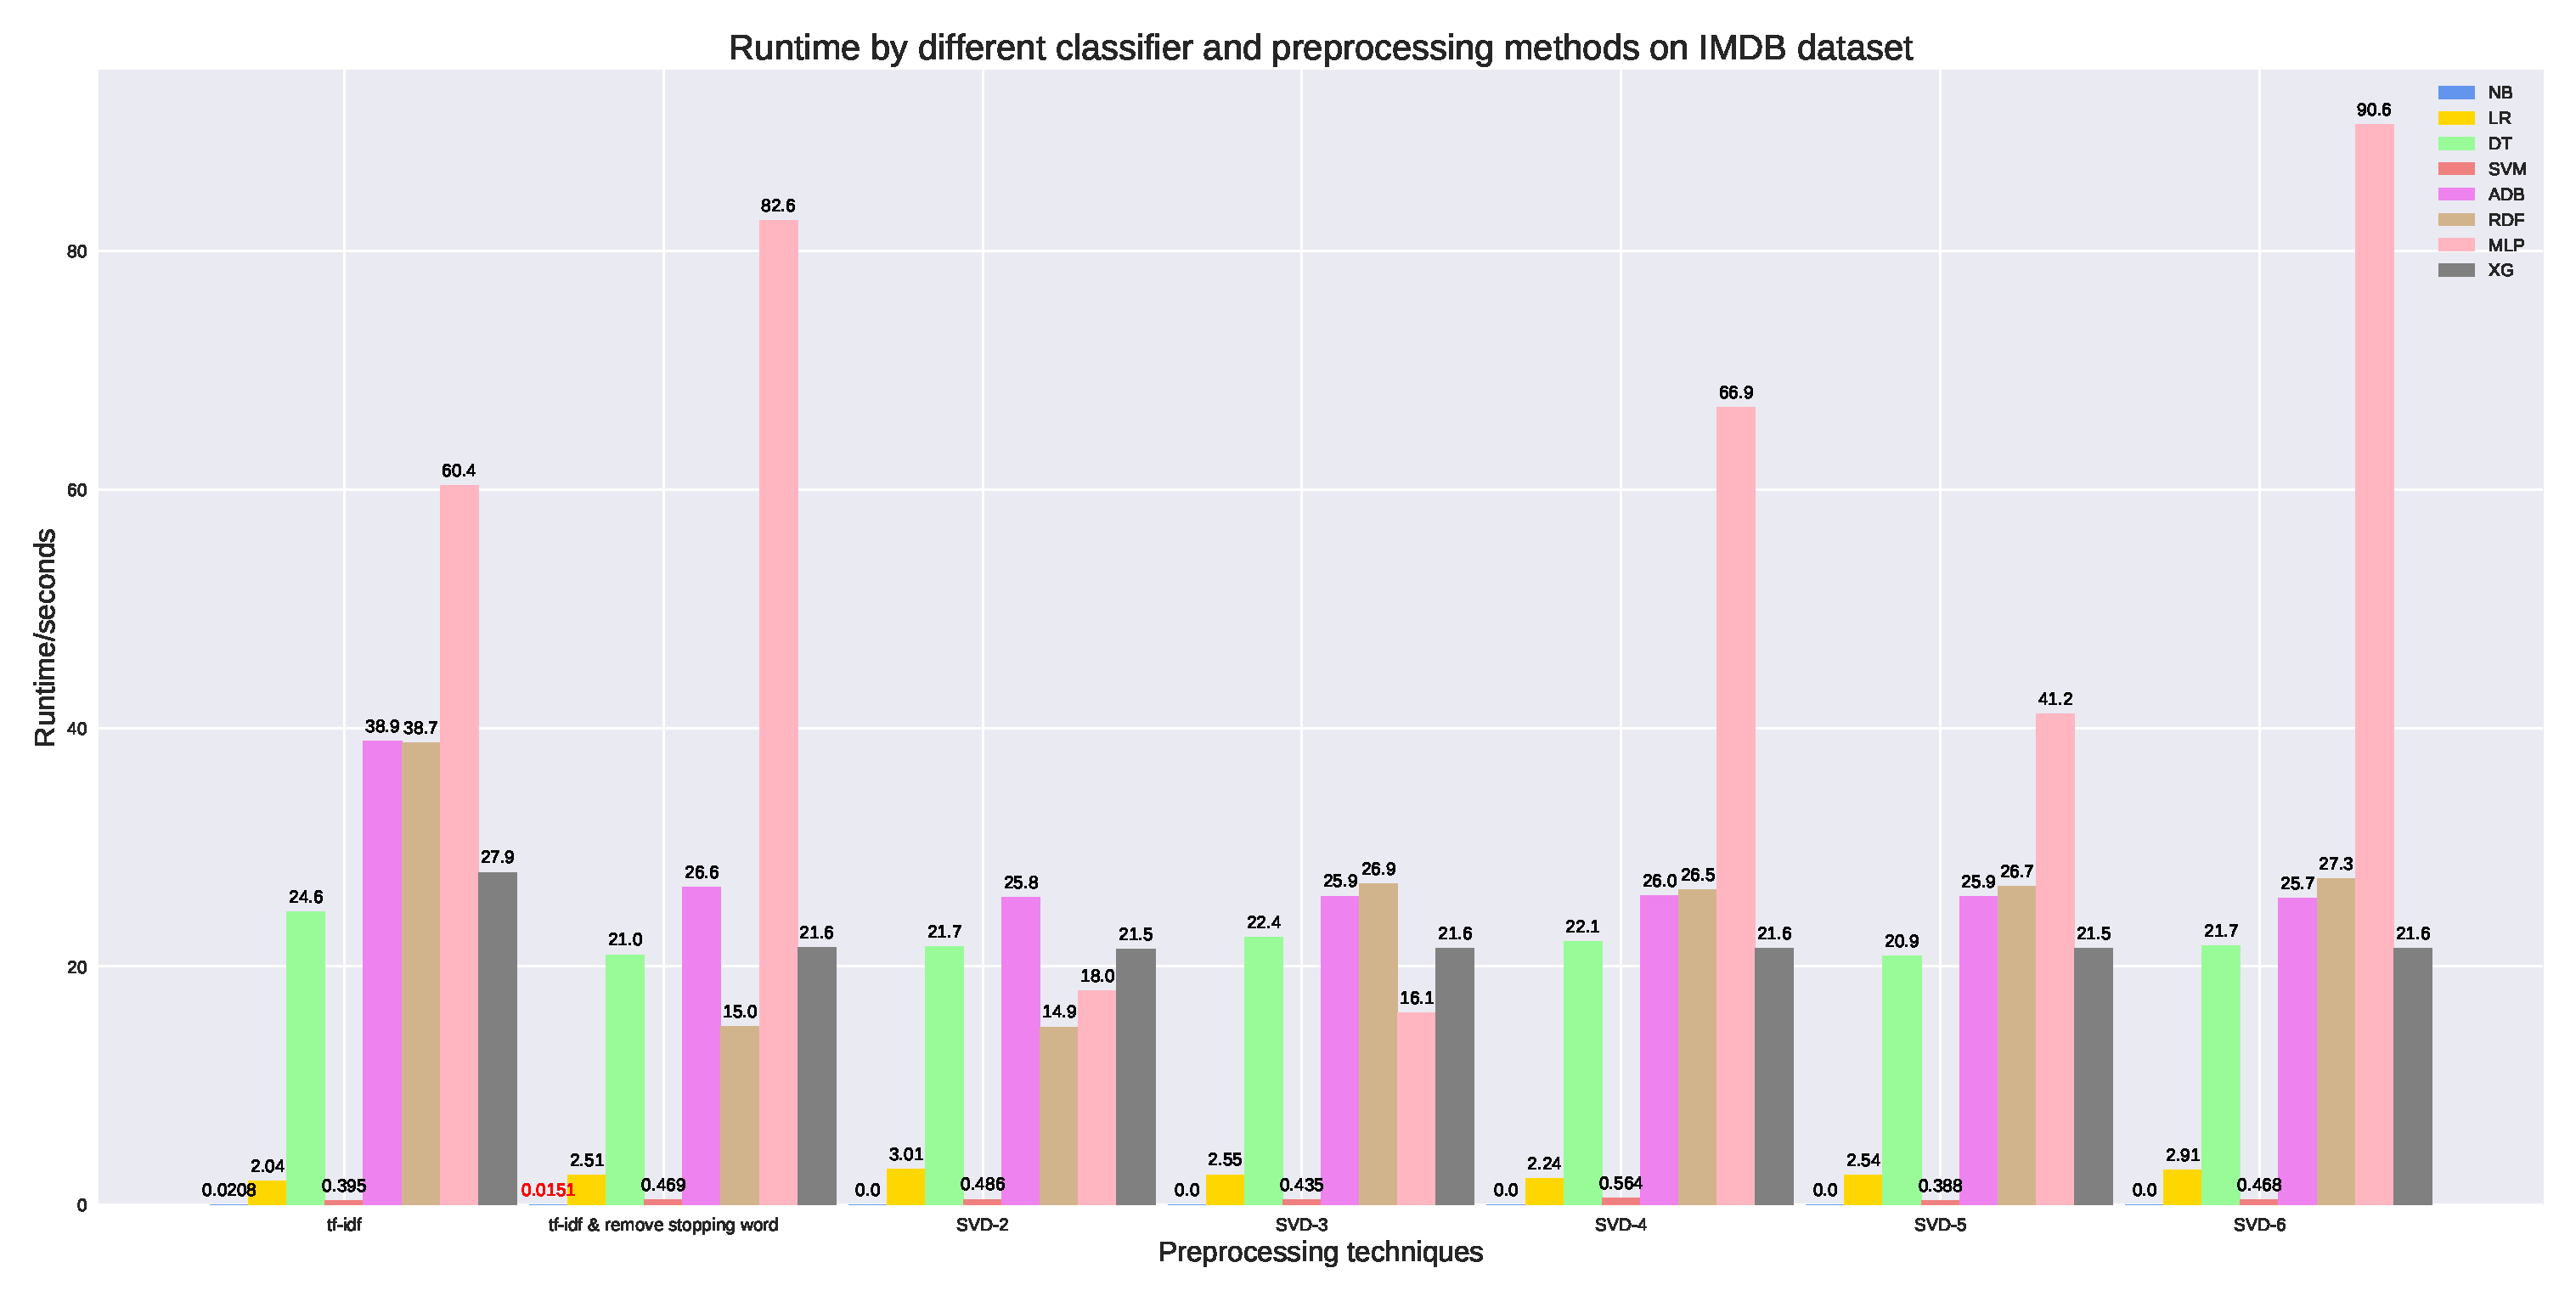
\includegraphics[width=0.9\linewidth]{fig/model_runtime_imdb.eps}
	\caption{Runtime performance on test dataset of IMDB dataset according to different pre-processing techniques}
	\label{runtime_imdb}
\end{figure}

We find that removing stopping words and dimensional reductions will generally reduce the runtime except that NB is influenced slightly and MLP's runtime will, in the contrary, have sharp increase. We find that NB has smallest runtime 0.0636 seconds in TF-IDF processed Twenty Newsgroup dataset and 0.0153 in TF-IDF \& removing stopping words IMDB dataset. Combined with the previous accuracy performance where TF-IDF preprocessing also outperforms, we deduce that more compressed representation like dimensional reductions will increase the information loss, which is harmful to our text classification, especially multi-label classification.

\subsubsection*{Best parameters}
It is costly to list best parameters for all preprocessing and model combinations, we only consider the best parameters of models on 'TF-IDF' processed datasets, since such preprocessing is best performed. The best parameters are listed in Table \ref{params}. We split the models into tunable and not-tunable ones. To be noticed that, we use term "not-tunable" because it is computationally heavy for the model to train so we roughly choose the best parameters manually. Most models have the same best parameters in two datasets, but NB, SVM and ADB have slight difference. The details of parameters tuning can be found in the output in \textit{Validation pipeline.ipynb}.

\begin{table}[H]
    \centering
    \begin{tabular}{c|cc}
        \hline
         &  Twenty Newsgroup  &  IMDB  \\
		\hline
		tunable & & \\
		\hline
        NB & alpha: 0.0, fit\_prior: True & alpha: 1.8, fit\_prior: True \\
		LR & penalty: 'l2', warm\_start: True & penalty: 'l2', warm\_start: True \\
		DT & criterion: 'gini', max\_features: None & criterion: 'gini', max\_features: None \\
		SVM & loss': 'squared\_hinge', penalty: 'l2' & loss': 'hinge', penalty: 'l2'\\
		ADB & learning\_rate: 0.6, n\_estimators: 100 & learning\_rate: 0.6, n\_estimators: 120 \\
		RDF & max\_depth: 60, n\_estimators: 150 & max\_depth: 60, n\_estimators: 150 \\
		\hline
		not tunable & & \\
		\hline
		MLP &  \multicolumn{2}{c}{hidden\_layer\_sizes: (30, 1024), max\_iter': 5000, solver: 'lbfgs' }  \\
		XG & \multicolumn{2}{c}{learning\_rate: 0.1}  \\
        \hline
    \end{tabular} 
    \caption{Best parameters of different classifiers using TF-IDF preprocessing technique on both datasets}
    \label{params}
\end{table}

\subsubsection*{Overall accuracy of different classifiers}
We also discuss the overall accuracy where we consider the true positive portion on two datasets' joint test result. The result is shown in Figure \ref{overall_accuracy}. We can find that only LR, SVM and MLP can outperform the baseline.

\begin{figure}[H]
	\centering
	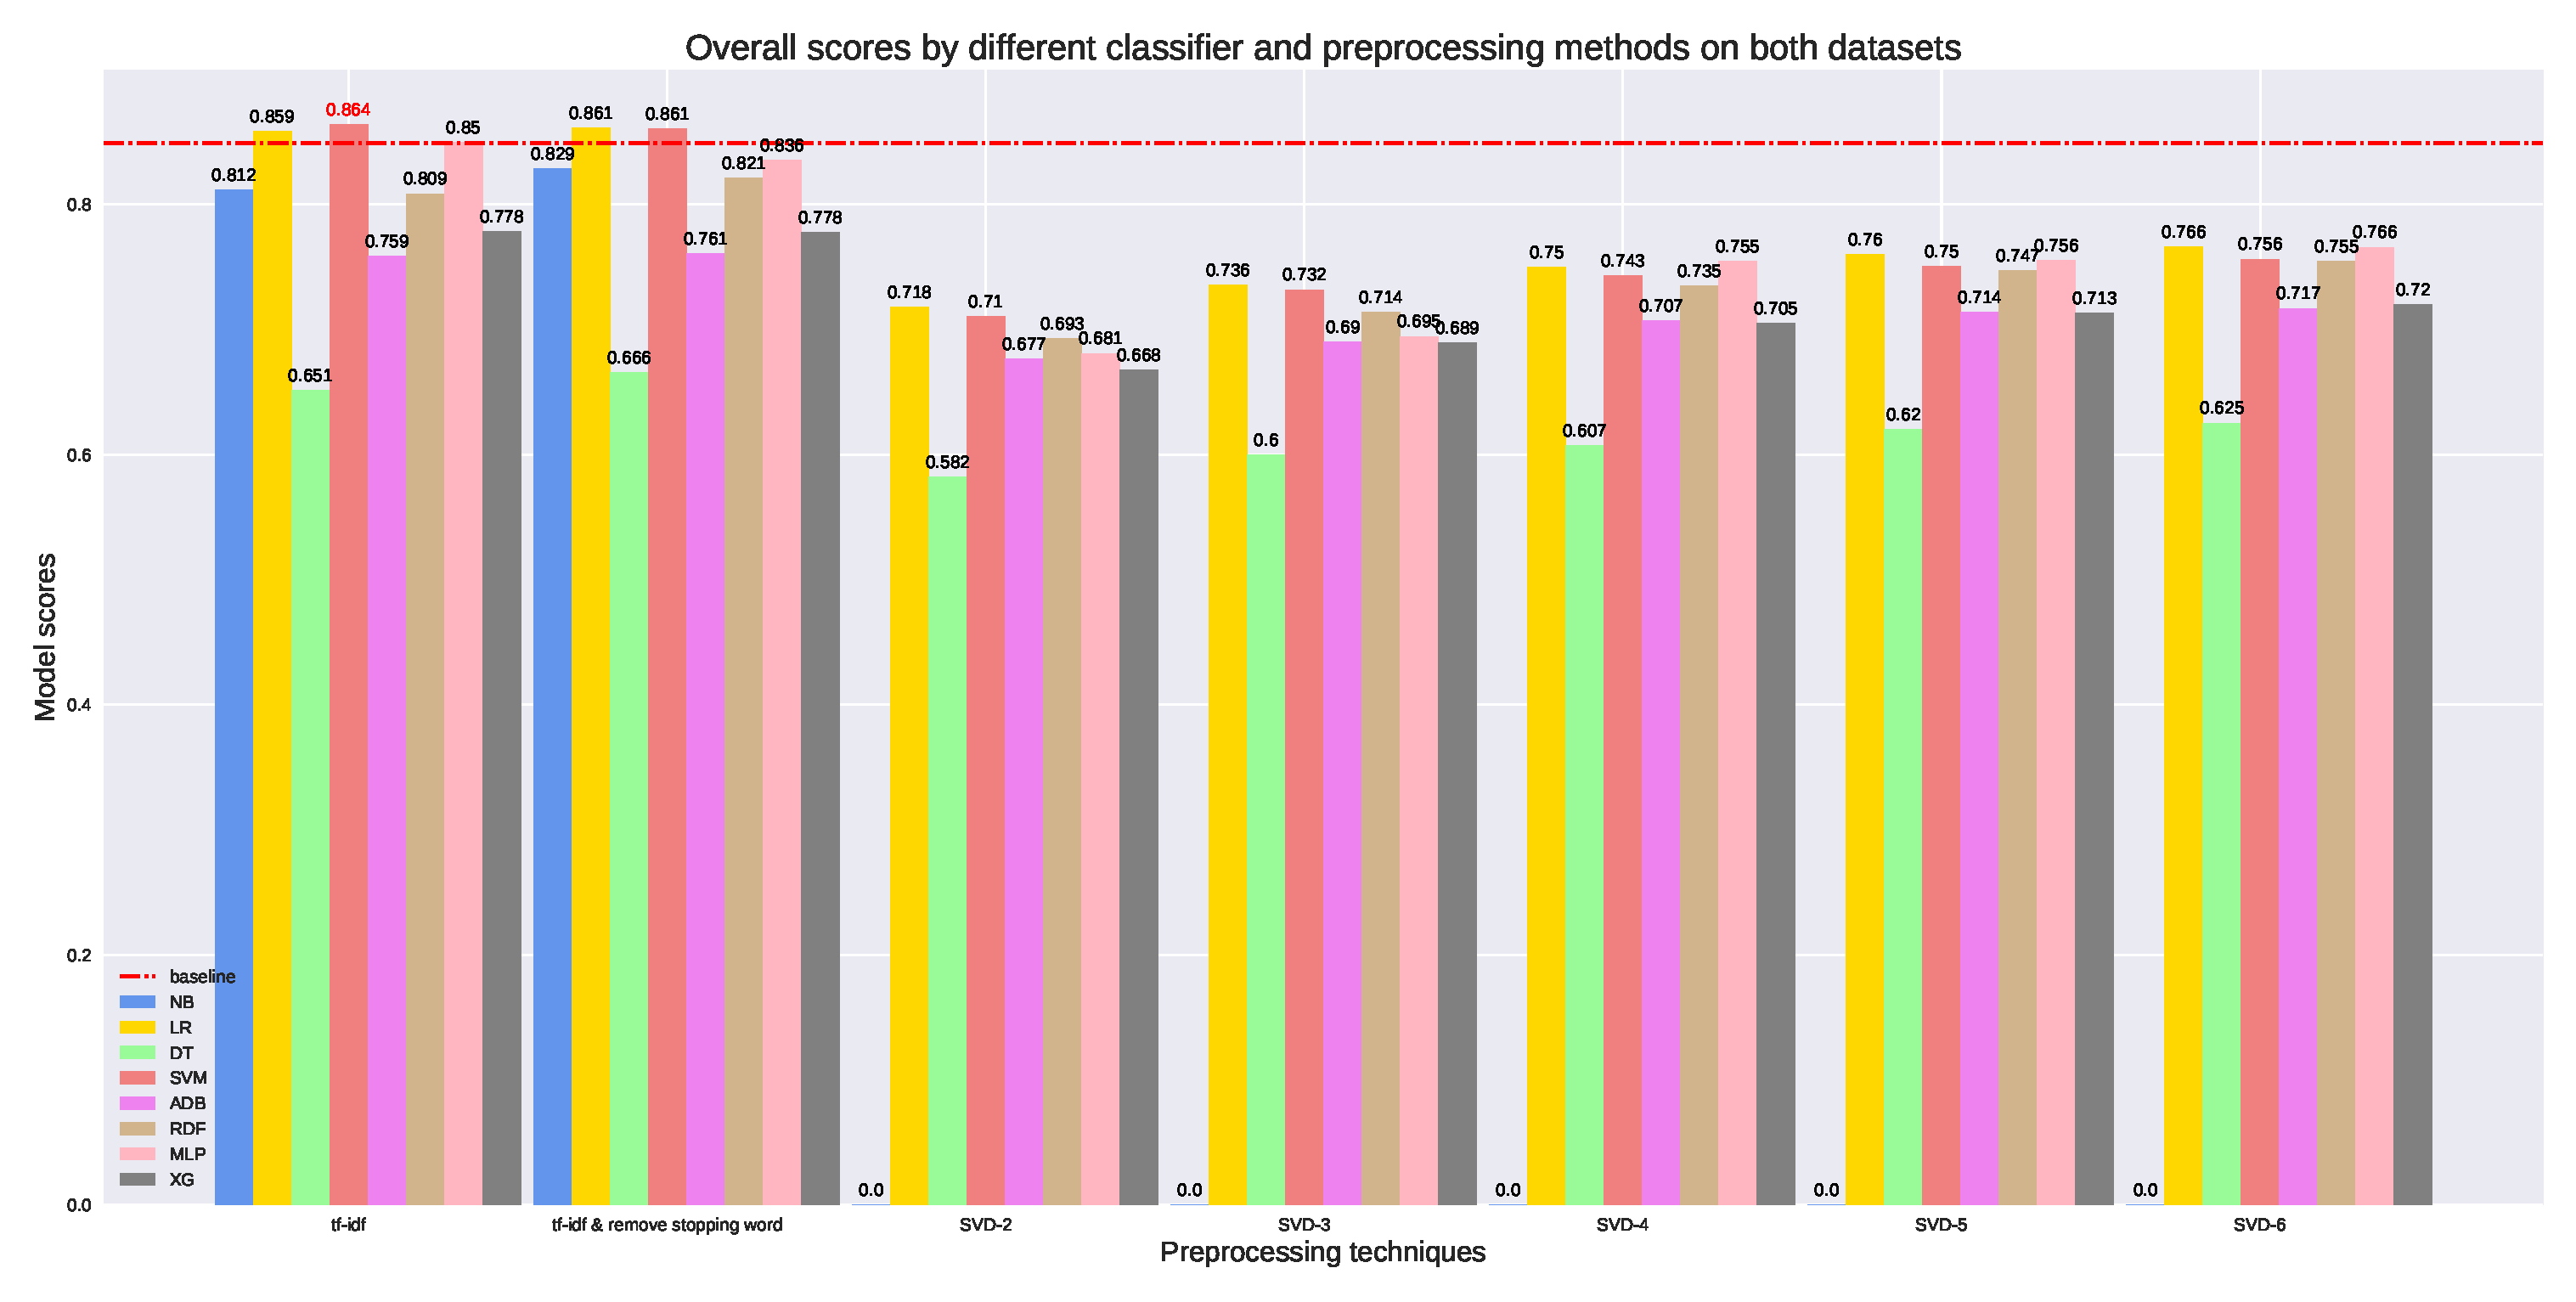
\includegraphics[width=0.9 \linewidth]{fig/model_acc_overall.eps}
	\caption{Overall accuracy performance on two datasets.}
	\label{overall_accuracy}
\end{figure}



\section{Discussion and Conclusion}
We outperform TA's baselines in Twenty Newsgroup dataset accuracy and overall accuracy and approximate very closely to IMDB dataset accuracy(ConvLSTM model on IMDB outperforms baseline a little bit [Table \ref{acc}]). We find that TF-IDF alone is very powerful preprocessing technique. Generally, SVM outperforms other classifiers and achieves highest accuracy in all cases. Runtime of traditional Machine Learning algorithm is much less than MLP based Neural Networks. Best parameters of models are roughly the same on two datasets but slightly differ. We also studied state-of-the-art method for higher accuracy. We constructed different LSTM structures (including BiLSTM\cite{graves2013hybrid}, ConvLSTM\cite{LSTM+CNN}) and analysed different hyper-parameters' effect. We found that convLSTM can improve the accuracy of vanilla LSTM model significantly on IMDB  dataset. However the accuracy drop down a bit in 20 news group dataset. Generally, ConvLSTM can speed up the training time approximate 50\%. For BiLSTM model, it has similar result on IMDB reviews dataset. But it will increase the accuracy of LSTM on 20 news group dataset in sacrifice of training time. The detailed results are given in Appendix.

\section{Statement for Contributions}
\begin{itemize}
	\item Fuyuan Lyu: Dataset preprocessing and feature engineering
	\item Tianyu Shi: Model design, hyper-parameter and model architecture analysis.
	\item Dingyi Zhuang: Experiments, validation pipelines and paper writing
\end{itemize}
\newpage
\bibliographystyle{unsrt}

\bibliography{ref}
\section{Appendix}
\subsection{Analysis of LSTM model}
\begin{itemize}
	\item Structure Results and Analysis
	Basically, we have analysed three different architectures of LSTM. Firstly, we consider the simple LSTM as shown in Figure \ref{LSTM}.
	\begin{figure}[H]
	\centering
	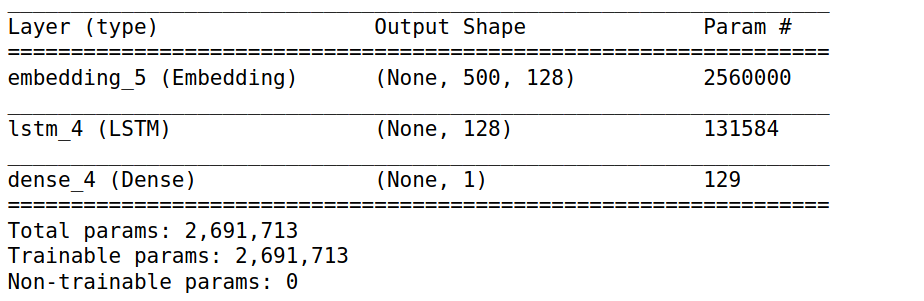
\includegraphics[width=0.9 \linewidth]{fig/lstm.png}
	\caption{Naive LSTM structure}
	\label{LSTM}
\end{figure}
	To improve our models performance, we further consider to apply CNN for feature embedding then use LSTM to do the sequence prediction, which is inspired from \cite{LSTM+CNN}, then we build the following model as shown in Figure \ref{ConvLSTM}.
	\begin{figure}[H]
	\centering
	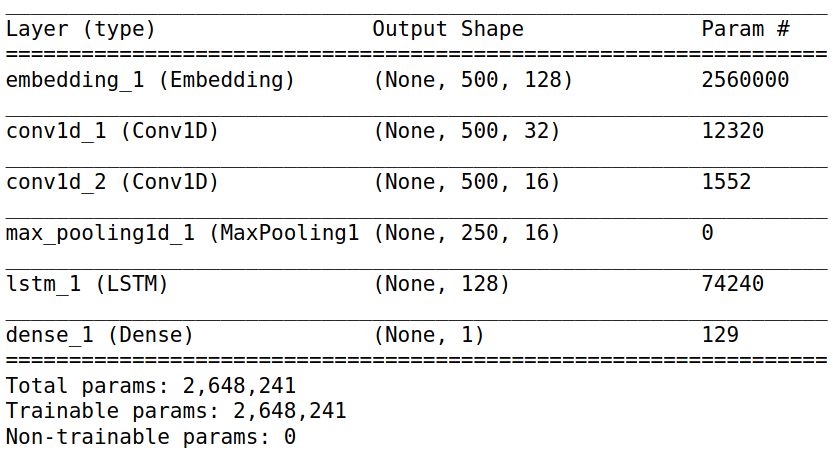
\includegraphics[width=0.6\linewidth]{fig/convlstm.png}
	\caption{ConvLSTM structure}
	\label{ConvLSTM}
\end{figure}
	Furthermore, to decrease the running time of our model, we modified the LSTM into biLSTM based on the best structure on each dataset, i.e. in IMDB dataset we use ConvbiLSTM and 20 news we use biLSTM. A typical structure of ConvbiLSTM is shown in Figure \ref{bilstm}.
	\begin{figure}[H]
	\centering
	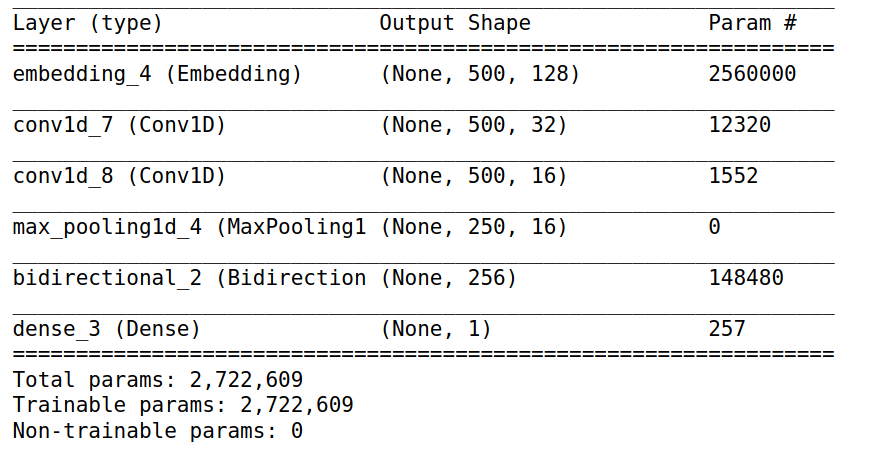
\includegraphics[width=0.7\linewidth]{fig/bilstm.png}
	\caption{biLSTM structure}
	\label{bilstm}
\end{figure}
The accuracy and run time of each model on different datasets are summarized in the following Table \ref{acc}.
% Please add the following required packages to your document preamble:
\begin{table}[H]
\centering
\begin{tabular}{|l|l|l|l|l|}
\hline
                 & &ConvLSTM  &LSTM  &BiLSTM    \\ \hline
\multirow{2}{*}{News} & Accuracy &0.6191  &0.6775  &0.6830  \\ \cline{2-5} 
                  &Runtime(s)  & 8314.1449 &15379.1084  &27298.4988  \\ \hline
\multirow{2}{*}{IMDB} & Accuracy &\textbf{0.8916}  &0.7533  &0.8844  \\ \cline{2-5} 
                  &Runtime(s)  &900.3511  &1767.4546  &1473.2600  \\ \hline
\end{tabular}
\label{acc}
\caption{Summary of different LSTM structures' accuracy and run time}
\end{table} 
	\item Hyper-parameter  Results and Analysis
	For hyper-parameter analysis, we firstly analysed the effect of max review length, we can find that the best parameter is 500, when the max review length is quite small, the accuracy turns to be very low.
	\begin{figure}[H]
	\centering
	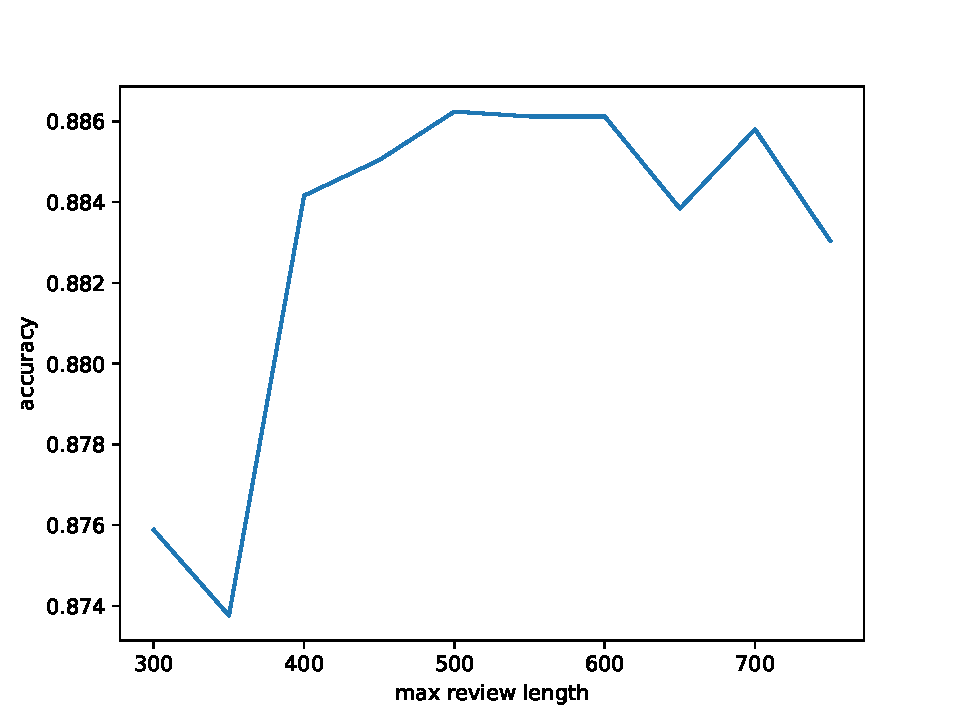
\includegraphics[width=0.7\linewidth]{fig/maxlen.pdf}
	\caption{Max review length's effect}
	\label{maxlen}
\end{figure}
	We have also analysed the effect of epoch in training, we found that for the smallest epoch the model has the highest accuracy on testing dataset, which is contrary to our hindsight, because more epochs should increase the accuracy a bit but will decrease the accuracy due to overfitting. We will further investigate the effect of drop-out parameter with epoch in the future.
	\begin{figure}[H]
	\centering
	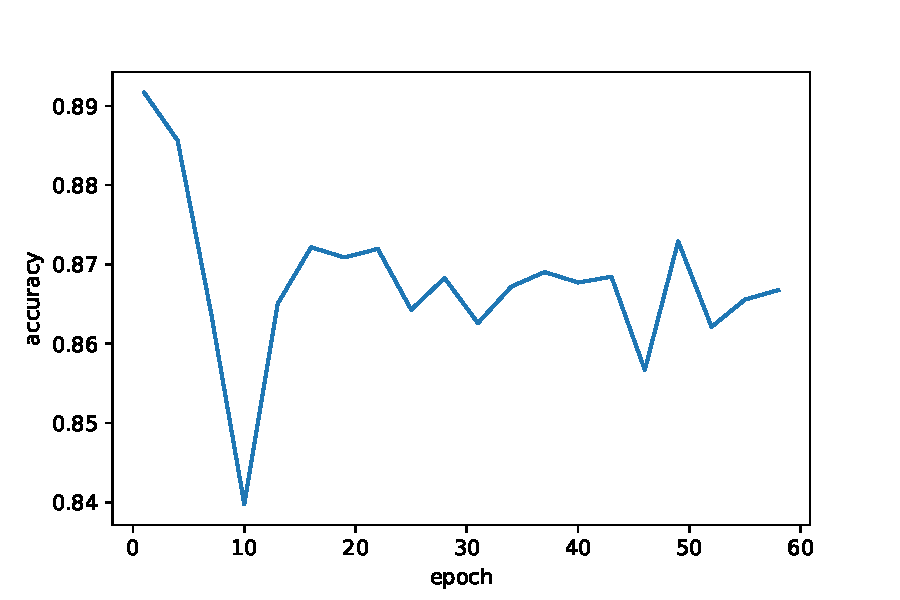
\includegraphics[width=0.7\linewidth]{fig/epoch.pdf}
	\caption{Epoch's effect}
	\label{epoch}
\end{figure}
\end{itemize}
\end{document}
